\documentclass[11pt]{article}
\usepackage[margin=.75in]{geometry}
\usepackage{amsmath,amssymb,amsthm,mathtools}
\usepackage{bbm}
\usepackage{graphicx}
\usepackage{booktabs}
\usepackage{enumitem}
\usepackage{tikz}
\usetikzlibrary{arrows.meta,positioning,shapes,fit}
\usepackage{pgfplots}
\pgfplotsset{compat=1.18}
\usepackage{longtable}
\usepackage{hyperref}
\usepackage[numbers,sort&compress]{natbib}

\hypersetup{
  colorlinks=true,
  linkcolor=blue,
  citecolor=blue,
  urlcolor=blue
}

% --- Macros ---
\newcommand{\RR}{\mathbb{R}}
\newcommand{\EE}{\mathbb{E}}
\newcommand{\PP}{\mathbb{P}}
\newcommand{\1}{\mathbbm{1}}

\newcommand{\ASCDE}{\mathrm{ASCDE}}
\newcommand{\RA}{\mathrm{RA}}
\newcommand{\ELCC}{\mathrm{ELCC}}
\newcommand{\LOLE}{\mathrm{LOLE}}
\newcommand{\EUE}{\ensuremath{\mathrm{EUE}}}
\newcommand{\VOLL}{\mathrm{VOLL}}
\newcommand{\LMP}{\mathrm{LMP}}
\newcommand{\CVaR}{\mathrm{CVaR}}

\newtheorem{assumption}{Assumption}
\newtheorem{proposition}{Proposition}
\newtheorem{lemma}{Lemma}
\newtheorem{definition_env}{Definition}
\newenvironment{definition}{\begin{definition_env}}{\end{definition_env}}
\newtheorem{remark}{Remark}

\title{%
Risk-Aware Locational Storage Bid Bounds and Reliability-Aware\\
Resource Valuation: An ASCDE/UEVF Perspective%
}

\author{Justin Candler
}

\date{%
As of: 2025--12--04
}

\begin{document}
\maketitle

\begin{abstract}
Battery storage is increasingly central to system reliability, energy arbitrage, and market-power debates in high-renewables grids.
Yet storage offers are governed by intertemporal opportunity costs under uncertainty, not fuel costs, making traditional offer caps and mitigation tools conceptually weak.
Recent work by Qi and Xu~\cite{QiXu2025} develops \emph{locational, state-of-charge--dependent storage bid bounds} derived from a tractable multi-period chance-constrained economic dispatch model.
These bounds are probabilistic caps on truthful marginal opportunity costs that scale with net-load uncertainty and the system operator's risk preference.

This paper develops a complementary perspective from the Unified Energy Valuation Framework (UEVF) and the system-aware cost of dependable energy (\(\ASCDE\)) paradigm.
We (i) formalize the link between chance-constrained dispatch, risk-aware locational marginal prices, and storage opportunity costs; (ii) embed Qi--Xu style bid bounds into the \(\ASCDE\) and reliability calculus used for planning and selection of resources; and (iii) articulate policy and implementation implications for ISO/RTOs considering storage offer caps that are coherent with explicit reliability and risk metrics.

We provide a unified view in which storage offer caps, reliability targets (\(\LOLE,\EUE\)), scarcity pricing, and planning metrics (ASCDE, marginal reliability value) arise as different slices of a single stochastic optimization problem rather than as independent institutional layers.
We also outline a set of appendices---including a full primal--dual formulation, distributionally robust uncertainty sets, and a stylized calibration from \(\varepsilon\) to \(\LOLE\)---that can support deeper technical and regulatory scrutiny.
\end{abstract}

\newpage

\tableofcontents

\newpage

\section{Introduction}

\subsection{Motivation}

In contemporary ISO/RTO markets, battery storage is no longer a marginal participant.
At penetrations on the order of 20--35\% of installed capacity, storage materially shapes:
\begin{itemize}[leftmargin=*]
  \item energy prices and congestion patterns,
  \item adequacy margins during net-load peaks, and
  \item the value and utilization of transmission upgrades and renewables.
\end{itemize}
At the same time, storage's economics are fundamentally intertemporal and state-of-charge (SoC) dependent:
its short-run ``marginal cost'' is an \emph{opportunity value} over future scarcity states, rather than a fuel-based scalar.

Traditional market power mitigation and offer-cap designs were inherited from a thermal-centric era.
They typically:
\begin{itemize}[leftmargin=*]
  \item specify static price caps (e.g., 1000--2000~\$/MWh),
  \item rely on cost-based offers tied to fuel and variable O\&M, or
  \item for storage, employ ad-hoc heuristics (e.g., ``4th-highest day-ahead LMP over the previous month'').
\end{itemize}
None of these constructions explicitly integrate:
\begin{enumerate}[leftmargin=*]
  \item net-load and renewable uncertainty,
  \item the operator's risk preference over constraint violations,
  \item or long-run reliability metrics (\(\LOLE, \EUE\)) and value-of-lost-load (\(\VOLL\)).
\end{enumerate}
The resulting caps can be simultaneously too high for some states (leaving market power unchecked) and too low for others (suppressing legitimate opportunity costs that support reliability).

Qi and Xu~\cite{QiXu2025} propose a step-change: derive \emph{locational, SoC-dependent storage bid bounds} from an explicit multi-period chance-constrained economic dispatch (CED) formulation.
In their setup:
\begin{itemize}[leftmargin=*]
  \item net-load uncertainty is modeled with minimal distributional assumptions;
  \item constraints are enforced with probability at least \(1-\varepsilon\), where \(\varepsilon\) is chosen by the system operator;
  \item dual variables on SoC and power balance constraints yield \emph{risk-aware} opportunity costs and LMPs;
  \item bid bounds are set to be high-probability envelopes for these opportunity costs.
\end{itemize}
Numerically, they show that such caps can:
\begin{itemize}[leftmargin=*]
  \item reduce system operating costs by \(\sim 0.1{-}0.5\%\),
  \item often increase storage profits in regimes with strong economic withholding, and
  \item preserve the ability of storage to capture legitimate scarcity rents in high-uncertainty environments.
\end{itemize}

In parallel, the Unified Energy Valuation Framework (UEVF) and the system-aware cost of dependable energy (\(\ASCDE\)) approach argue that planning and resource selection should be grounded in:
\begin{itemize}[leftmargin=*]
  \item explicit reliability metrics (\(\LOLE, \EUE\)),
  \item capacity credit via effective load-carrying capability (\(\ELCC\)),
  \item and monetization of reliability shortfalls via \(\VOLL\).
\end{itemize}
The core idea is that resource economics should be evaluated on a \emph{dependable energy} basis, not raw MWh, and that reliability should be internalized into resource costs, not treated as an external check.

This paper's central thesis is that these two strands---risk-aware storage bid bounds and reliability-aware valuation via \(\ASCDE\)---are natural complements.
The same stochastic structure that yields risk-aware LMPs and storage opportunity costs should drive:
\begin{itemize}[leftmargin=*]
  \item scarcity pricing,
  \item reliability metrics (\(\LOLE,\EUE\)),
  \item and the numerator/denominator of \(\ASCDE\).
\end{itemize}
Storage bid caps then become a constrained interface between operational risk preferences and planning-side reliability targets, rather than an arbitrary regulatory artifact.

\subsection{Contributions and scope}

We focus on three main tasks:
\begin{enumerate}[leftmargin=*]
  \item \textbf{Formalization of the CED--ASCDE link.}
  We restate the Qi--Xu chance-constrained multi-period dispatch in a planner-centric language and explicitly connect:
  \begin{itemize}
    \item risk-aware LMPs and SoC shadow prices, and
    \item reliability metrics and \(\ASCDE\).
  \end{itemize}
  This clarifies the interpretation of storage bid bounds as caps on \(\VOLL\)-consistent opportunity costs.

  \item \textbf{Embedding bid bounds into UEVF/ASCDE.}
  We develop a conceptual optimization problem where:
  \begin{itemize}
    \item the CED risk parameter \(\varepsilon\) and uncertainty scaling control short-run dispatch and bid bounds, and
    \item long-run reliability constraints (target \(\LOLE^\star, \EUE^\star\)) and \(\ASCDE\) drive portfolio choice.
  \end{itemize}
  We argue that the choice of \(\varepsilon\) should be calibrated to reliability targets, not chosen in isolation.

  \item \textbf{Policy and implementation map.}
  We outline a concrete implementation pathway for ISO/RTOs that:
  \begin{itemize}
    \item replaces heuristic storage caps with locational, SoC-dependent qi--Xu-style bounds,
    \item aligns scarcity pricing and \(\VOLL\), and
    \item exposes the risk policy knob \(\varepsilon\) to regulators and stakeholders in a transparent way.
  \end{itemize}
\end{enumerate}

We do \emph{not} attempt to:
\begin{itemize}[leftmargin=*]
  \item reproduce Qi and Xu's full numerical case studies,
  \item implement a full production-level CED solver, or
  \item resolve all design choices around scarcity pricing and uplift.
\end{itemize}
Instead, we focus on the structural relationships that should guide such implementations.

\subsection{Notation and conventions}

We keep notation close to Qi--Xu where convenient but adapt to a planning perspective.

\begin{itemize}[leftmargin=*]
  \item Time periods: \(t \in \mathcal{T} = \{1,\dots,T\}\).
  \item Nodes/buses: \(n \in \mathcal{N}\).
  \item Generators: \(i \in G\); storage units: \(s \in S\).
  \item Net-load: random vector \(\tilde{d} = (\tilde{d}_{n,t})_{n,t}\) with mean \(d\) and dispersion parameters \(\sigma_{n,t}\).
  \item LMPs: \(\lambda_{n,t}\) in deterministic ED; \(\hat{\lambda}_{n,t}\) (or \(\hat{\LMP}_{n,t}\)) in CED.
  \item SoC shadow values: \(\theta_{s,t}\) (deterministic) and \(\hat{\theta}_{s,t}\) (risk-aware).
  \item Storage SoC: \(e_{s,t}\); normalized SoC \(\xi_{s,t} := (e_{s,t} - \underline{e}_s) / (\overline{e}_s - \underline{e}_s) \in [0,1]\).
  \item Risk parameter: \(\varepsilon \in (0,1)\) in chance constraints.
\end{itemize}

We adopt the convention that expectations \(\EE[\cdot]\) and probabilities \(\PP(\cdot)\) are taken with respect to the net-load stochastic process and any other modeled uncertainties unless otherwise noted.

\section{Reliability Metrics and ASCDE}

This section develops the reliability and \(\ASCDE\) concepts we will later link to CED and storage bid bounds.

\subsection{Reliability metrics}

We consider a standard probabilistic adequacy model:
\begin{itemize}[leftmargin=*]
  \item load is a stochastic process \(L_t\),
  \item generation (including renewables and storage) has stochastic availability,
  \item contingency events (forced outages) follow specified distributions.
\end{itemize}

We focus on two metrics:
\begin{description}[leftmargin=*,style=nextline]
  \item[\(\LOLE\) (loss of load expectation).]
    The expected number of periods (typically days or hours) in which demand exceeds available supply over a given horizon (e.g., a year).
    For hourly modeling:
    \[
      \LOLE = \sum_{t=1}^T \PP\big( L_t > \text{available capacity}_t \big).
    \]
  \item[\(\EUE\) (expected unserved energy).]
    The expected energy not served over the horizon:
    \[
      \EUE = \sum_{t=1}^T \EE\big[ (L_t - \text{available capacity}_t)_+ \big],
    \]
    where \((x)_+ := \max\{x,0\}\).
\end{description}
These can be computed via Monte Carlo simulation or analytically in simplified models.

Given a portfolio \(R\) of resources (including storage), we denote by \(\LOLE(R)\) and \(\EUE(R)\) the reliability metrics under that portfolio.

\subsection{Monetizing reliability via \texorpdfstring{\(\VOLL\)}{VOLL}}

Following standard practice, we monetize \(\EUE\) via a value-of-lost-load \(\VOLL\) (in \$/MWh).
The annual monetized reliability cost is:
\begin{equation}
  \RA(R)
  \;=\;
  \VOLL \cdot \EUE(R).
  \label{eq:RA-def}
\end{equation}
One may normalize by annual energy served \(E_{\mathrm{year}}(R)\) to get a per-MWh reliability cost:
\begin{equation}
  \RA_{\mathrm{perMWh}}(R)
  \;=\;
  \frac{\VOLL \cdot \EUE(R)}{E_{\mathrm{year}}(R)}.
\end{equation}

\subsection{System-aware cost of dependable energy}

Let \(R\) denote a resource portfolio.
We define:
\begin{itemize}[leftmargin=*]
  \item \(\mathrm{Capex}(R)\): annualized capital cost of the portfolio,
  \item \(\mathrm{FOM}(R)\): fixed O\&M,
  \item \(\mathrm{VOM}(R)\): variable O\&M and fuel,
  \item \(\mathrm{Tx}(R)\): transmission and interconnection costs,
  \item \(\mathrm{Sto}(R)\): storage-specific fixed and degradation costs,
  \item \(\RA(R)\): reliability cost from~\eqref{eq:RA-def},
  \item \(E_{\mathrm{rel}}(R)\): \emph{reliably deliverable energy} (MWh) over the horizon.
\end{itemize}

A canonical definition of the system-aware cost of dependable energy is:
\begin{equation}
  \ASCDE(R)
  \;=\;
  \frac{
    \mathrm{Capex}(R)
    + \mathrm{FOM}(R)
    + \mathrm{VOM}(R)
    + \mathrm{Tx}(R)
    + \mathrm{Sto}(R)
    + \RA(R)
  }{
    E_{\mathrm{rel}}(R)
  }.
  \label{eq:ASCDE-def}
\end{equation}
In practice, \(E_{\mathrm{rel}}(R)\) is computed as:
\[
  E_{\mathrm{rel}}(R)
  = \sum_{r \in R} \ELCC_r \cdot E_r,
\]
where \(\ELCC_r \in [0,1]\) is the effective load-carrying capability of resource \(r\) (fraction of its nameplate capacity that counts as firm) and \(E_r\) its expected energy deliveries.

\subsection{Marginal reliability value}

For a given portfolio \(R\) and candidate incremental resource \(r\), we define a marginal reliability value (MRV) at increment \(\Delta q\) MW as:
\begin{equation}
  \mathrm{MRV}_r(R; \Delta q)
  := 
  - \VOLL \cdot \frac{\EUE(R \cup \{r(\Delta q)\}) - \EUE(R)}{\Delta q},
  \label{eq:MRV-fd}
\end{equation}
where \(r(\Delta q)\) denotes an increment of \(r\) of size \(\Delta q\).
In the continuous limit, we write:
\begin{equation}
  \mathrm{MRV}_r(R)
  := - \VOLL \cdot \frac{\partial \EUE(R)}{\partial q_r}.
  \label{eq:MRV-deriv}
\end{equation}
This quantity (in \$/MW-year) is directly comparable to the annualized cost per MW of capacity, and supports ranking resources by net value per unit of reliability impact.

Storage's MRV depends on:
\begin{itemize}[leftmargin=*]
  \item its power rating (MW),
  \item its energy duration (MWh),
  \item its efficiency, and
  \item its correlation with existing renewables and load.
\end{itemize}
Crucially, MRV is \emph{not} a static number: it changes with the portfolio \(R\) and with the scarcity structure induced by network constraints and demand patterns.

\section{Chance-Constrained Economic Dispatch with Storage}

We now develop the chance-constrained multi-period dispatch problem and its dual structure.

\begin{figure}[t]
  \centering
  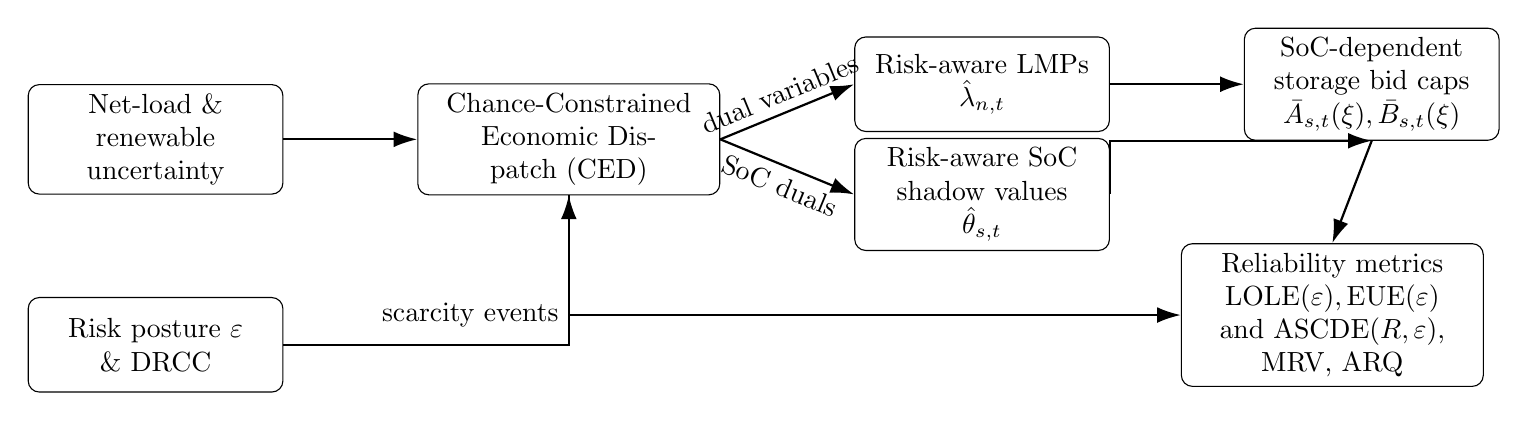
\begin{tikzpicture}[
    node distance=1.3cm and 1.7cm,
    box/.style={rectangle, draw, rounded corners, align=center, text width=3cm, minimum height=1.2cm},
    bigbox/.style={rectangle, draw, rounded corners, align=center, text width=3.6cm, minimum height=1.4cm},
    arrow/.style={-{Latex[length=3mm,width=2mm]}, thick}
  ]

    \node[box] (unc) {Net-load \&\\renewable uncertainty};
    \node[box, below=of unc] (risk) {Risk posture $\varepsilon$\\\& DRCC};

    \node[bigbox, right=of unc] (ced) {Chance-Constrained Economic Dispatch (CED)};

    \node[box, right=of ced, yshift=0.7cm] (lmp) {Risk-aware LMPs\\$\hat{\lambda}_{n,t}$};
    \node[box, right=of ced, yshift=-0.7cm] (soc) {Risk-aware SoC shadow values\\$\hat{\theta}_{s,t}$};

    \node[box, right=of lmp] (bids) {SoC-dependent storage bid caps\\$\bar{A}_{s,t}(\xi), \bar{B}_{s,t}(\xi)$};

    \node[bigbox, below=of bids, xshift=-0.5cm] (ascde) {Reliability metrics $\LOLE(\varepsilon),\EUE(\varepsilon)$\\and $\ASCDE(R,\varepsilon)$, MRV, ARQ};

    % arrows unchanged ...
    \draw[arrow] (unc.east) -- (ced.west);
    \draw[arrow] (risk.east) -| (ced.south);

    \draw[arrow] (ced.east) -- node[above,sloped]{dual variables} (lmp.west);
    \draw[arrow] (ced.east) -- node[below,sloped]{SoC duals} (soc.west);

    \draw[arrow] (lmp.east) -- (bids.west);
    \draw[arrow] (soc.east) |- (bids.south);

    \draw[arrow] (ced.south) |- node[left,sloped]{scarcity events} (ascde.west);
    \draw[arrow] (bids.south) -- (ascde.north);

  \end{tikzpicture}
  \caption{Conceptual architecture linking chance-constrained economic dispatch (CED),
  risk-aware LMPs and SoC shadow values, storage bid caps, and reliability-aware
  valuation metrics such as $\LOLE(\varepsilon)$, $\EUE(\varepsilon)$, and
  $\ASCDE(R,\varepsilon)$.}
  \label{fig:architecture}
\end{figure}

\subsection{Deterministic multi-period DC-OPF with storage}

We start with the deterministic case, closely aligned with standard DC-OPF formulations.

\subsubsection{Primal problem}

Let:
\begin{itemize}[leftmargin=*]
  \item \(g_{i,t}\) be generation output of unit \(i \in G\) at time \(t\),
  \item \(p_{s,t}\) and \(b_{s,t}\) be discharge and charge power of storage unit \(s \in S\),
  \item \(e_{s,t}\) be SoC of storage,
  \item \(f_{\ell,t}\) be power flow on line \(\ell\),
  \item \(d_{n,t}\) be deterministic net demand at node \(n\).
\end{itemize}

The deterministic multi-period economic dispatch (ED) problem is:
\begin{equation}
  \begin{aligned}
  \min_{g,p,b,e,f}
  \quad
  & \sum_{t=1}^T \left( 
    \sum_{i \in G} C_i(g_{i,t}) 
    + \sum_{s \in S} M_s (p_{s,t} + b_{s,t})
  \right) \\
  \text{s.t.} \quad
  & \text{Power balance:} \\
  & \sum_{i \in G_n} g_{i,t}
    + \sum_{s \in S_n} (p_{s,t} - b_{s,t})
    - d_{n,t}
    = \sum_{\ell \in \mathcal{L}_n} f_{\ell,t},
    \quad \forall n,t, \\
  & \text{Line limits:} \\
  & -\overline{F}_\ell \le f_{\ell,t} \le \overline{F}_\ell, \quad \forall \ell,t, \\
  & \text{DC flow:} \\
  & f_{\ell,t} = \sum_{n} H_{\ell n} \theta_{n,t}^{\text{ang}}, \quad \forall \ell,t, \\
  & \text{Generator limits and ramps:} \\
  & \underline{g}_i \le g_{i,t} \le \overline{g}_i, \quad \forall i,t, \\
  & |g_{i,t} - g_{i,t-1}| \le R_i, \quad \forall i,t, \\
  & \text{Storage SoC dynamics:} \\
  & e_{s,t+1} = e_{s,t} + \eta_s b_{s,t} - \frac{1}{\eta_s} p_{s,t},
    \quad \forall s,t, \\
  & \underline{e}_s \le e_{s,t} \le \overline{e}_s, \quad \forall s,t, \\
  & 0 \le b_{s,t} \le \overline{b}_s, \quad 0 \le p_{s,t} \le \overline{p}_s, \quad \forall s,t.
  \end{aligned}
  \label{eq:det-ED-full}
\end{equation}
We suppress voltage angle reference and ancillary service constraints for brevity.

\subsubsection{Dual variables and storage opportunity cost}

Let:
\begin{itemize}[leftmargin=*]
  \item \(\lambda_{n,t}\) be the dual multiplier of the power-balance constraint at node \(n\), time \(t\); this is the LMP.
  \item \(\mu_{s,t}\) be the dual multiplier associated with the SoC balance constraint for storage unit \(s\), time \(t\).
\end{itemize}
The storage-related Lagrangian terms are:
\[
  \mathcal{L}_{\mathrm{sto}}
  =
  \sum_{t,s}
  \Big(
    M_s (p_{s,t} + b_{s,t})
    + \mu_{s,t} (e_{s,t+1} - e_{s,t} - \eta_s b_{s,t} + \tfrac{1}{\eta_s} p_{s,t})
    - \lambda_{n(s),t} (p_{s,t} - b_{s,t})
  \Big)
  + \cdots
\]
Differentiating with respect to \(p_{s,t}\) and \(b_{s,t}\) and imposing KKT conditions yields:
\begin{subequations}
\begin{align}
  \frac{\partial \mathcal{L}_{\mathrm{sto}}}{\partial p_{s,t}}
  &= M_s + \mu_{s,t} \tfrac{1}{\eta_s} - \lambda_{n(s),t} + \cdots = 0, \\
  \frac{\partial \mathcal{L}_{\mathrm{sto}}}{\partial b_{s,t}}
  &= M_s - \mu_{s,t} \eta_s + \lambda_{n(s),t} + \cdots = 0,
\end{align}
\end{subequations}
for marginal units (i.e., where power or SoC limits are not binding).

Define:
\begin{subequations}
\begin{align}
  A_{s,t} &:= M_s + \frac{\mu_{s,t}}{\eta_s}, \\
  B_{s,t} &:= \mu_{s,t} \eta_s - M_s.
\end{align}
\end{subequations}
At an interior optimum, \(A_{s,t} = \lambda_{n(s),t}\) when storage is discharging and \(B_{s,t} = -\lambda_{n(s),t}\) when charging, capturing the fact that marginal opportunity cost is aligned with LMP in a frictionless competitive equilibrium.

Qi and Xu use an equivalent notation with \(\theta_{s,t}\) for the SoC shadow value; we will follow their convention and write:
\begin{subequations}
\begin{align}
  A_{s,t} &:= M_s + \frac{\theta_{s,t}}{\eta_s}, \label{eq:A-det}\\
  B_{s,t} &:= \theta_{s,t} \eta_s - M_s. \label{eq:B-det}
\end{align}
\end{subequations}
Here, \(\theta_{s,t}\) is the marginal value of one extra unit of SoC at time \(t\), in the deterministic ED.

\subsection{Chance-constrained ED with net-load uncertainty}

Now let net-load be random: \(\tilde{d}_{n,t}\).
We assume:
\begin{assumption}[Net-load uncertainty structure]
\label{ass:netload}
For each \(t\), the net-load vector \(\tilde{d}_{\cdot,t}\) has mean \(d_{\cdot,t}\) and centered variation \(\tilde{z}_{\cdot,t} := \tilde{d}_{\cdot,t} - d_{\cdot,t}\) belonging to a distributionally specified set \(\mathcal{U}_t\).
Uncertainty across times may be correlated, but we assume that suitable second-moment (or robust) bounds are available for each linear combination of \(\tilde{z}\) appearing in constraints.
\end{assumption}

Key constraints (line limits, reserve requirements, etc.) depend linearly on \(\tilde{d}\).
A generic chance constraint takes the form:
\begin{equation}
  \PP\big( a^\top x + c^\top \tilde{z} \le b \big)
  \;\ge\; 1 - \varepsilon,
  \label{eq:generic-cc}
\end{equation}
for some deterministic decision variables \(x\) and random vector \(\tilde{z}\).

Qi and Xu consider several tractable approximations to~\eqref{eq:generic-cc}, including:
\begin{itemize}[leftmargin=*]
  \item assuming sub-Gaussian or light-tailed bounds,
  \item using Cantelli or Chebyshev inequalities,
  \item and distributionally robust sets defined by moment and shape constraints.
\end{itemize}
In each case,~\eqref{eq:generic-cc} is conservatively approximated by a deterministic constraint of the form:
\begin{equation}
  a^\top x + \kappa(\varepsilon) \cdot \sigma_{\mathrm{eff}} \le b,
  \label{eq:cc-deterministic}
\end{equation}
where \(\sigma_{\mathrm{eff}}\) is an effective standard deviation and \(\kappa(\varepsilon)\) a risk-sensitivity factor.

Replacing all relevant chance constraints in ED with approximations of type~\eqref{eq:cc-deterministic} yields the CED problem.
Solving it gives risk-aware dual variables:
\begin{itemize}[leftmargin=*]
  \item \(\hat{\lambda}_{n,t}\): risk-aware LMP at node \(n\), time \(t\),
  \item \(\hat{\theta}_{s,t}\): risk-adjusted SoC shadow value,
\end{itemize}
and associated marginal costs:
\begin{subequations}
\begin{align}
  \hat{A}_{s,t} &:= M_s + \frac{\hat{\theta}_{s,t}}{\eta_s}, \\
  \hat{B}_{s,t} &:= \hat{\theta}_{s,t} \eta_s - M_s.
\end{align}
\end{subequations}

\section{Risk-Aware Storage Bid Bounds}

We now develop the construction and properties of locational, SoC-dependent storage bid bounds.

\begin{figure}[t]
  \centering
  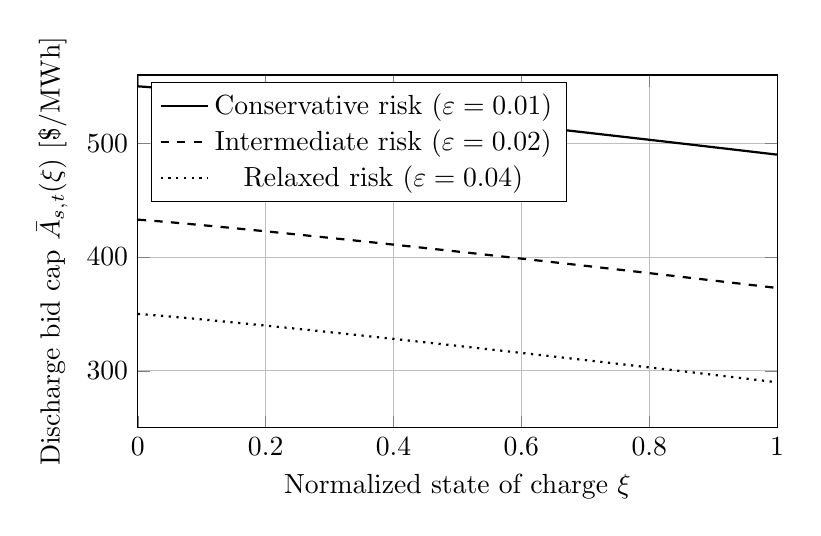
\begin{tikzpicture}
    \begin{axis}[
      width=0.8\textwidth,
      height=0.5\textwidth,
      xlabel={Normalized state of charge $\xi$},
      ylabel={Discharge bid cap $\bar{A}_{s,t}(\xi)$ [\$/MWh]},
      xmin=0, xmax=1,
      ymin=250, ymax=560,
      legend style={at={(0.02,0.98)},anchor=north west},
      grid=both,
      domain=0:1,
      samples=200
    ]
      % Conservative risk (epsilon = 0.01)
      \addplot[thick] {550 - 60*x^(1.1)};
      \addlegendentry{Conservative risk ($\varepsilon=0.01$)};

      % Medium risk (epsilon = 0.02)
      \addplot[thick, dashed] {432.8427124746 - 60*x^(1.1)};
      \addlegendentry{Intermediate risk ($\varepsilon=0.02$)};

      % Relaxed risk (epsilon = 0.04)
      \addplot[thick, dotted] {350 - 60*x^(1.1)};
      \addlegendentry{Relaxed risk ($\varepsilon=0.04$)};
    \end{axis}
  \end{tikzpicture}
  \caption{Illustrative SoC-dependent discharge bid caps $\bar{A}_{s,t}(\xi)$
  under three risk postures. The caps are monotonically decreasing in normalized
  state of charge $\xi$, and are higher under more conservative risk (smaller
  $\varepsilon$). All curves are generated from the same toy functional form
  $\bar{A}(\xi;\varepsilon) \approx 150 + 40/\sqrt{\varepsilon} - 60\xi^{1.1}$.}
  \label{fig:soc_bid_caps}
\end{figure}

\subsection{Probabilistic bid caps on opportunity cost}

The key design principle in Qi and Xu is:

\begin{definition}[Chance-constrained bid bounds]
For a chosen tolerance \(\varepsilon \in (0,1)\), discharge and charge bid bounds \(\bar{A}_{s,t}\), \(\bar{B}_{s,t}\) are said to be \emph{chance-constrained bid bounds} if they satisfy:
\begin{subequations}
\begin{align}
  \PP\big( \hat{A}_{s,t} \le \bar{A}_{s,t} \big) &\ge 1 - \varepsilon, \label{eq:bid-bound-chance-A}\\
  \PP\big( \hat{B}_{s,t} \le \bar{B}_{s,t} \big) &\ge 1 - \varepsilon. \label{eq:bid-bound-chance-B}
\end{align}
\end{subequations}
\end{definition}

Interpretation: with probability at least \(1-\varepsilon\), the ``truthful'' marginal opportunity cost of storage in CED lies below the cap.
Therefore, when a unit is cleared, any observed bid exceeding the cap is \emph{unlikely} to correspond to truthful marginal cost and may be treated as a market-power indicator.

Qi and Xu show that bid bounds can be constructed using envelopes of risk-aware LMPs.
In particular, under appropriate assumptions and normalizations, one can set:
\begin{subequations}
\begin{align}
  \bar{A}_{s,t}
  &= \max_{m} \hat{\LMP}_{m,t}, \\
  \bar{B}_{s,t}
  &= \min_{m} \hat{\LMP}_{m,t}.
\end{align}
\end{subequations}
We omit some intermediate derivation details here and instead focus on structural properties.

\subsection{SoC dependence and convexity}

Qi and Xu's numerical findings show that \(\bar{A}_{s,t}\) and \(\bar{B}_{s,t}\), when expressed as functions of normalized SoC \(\xi_{s,t}\), are:
\begin{itemize}[leftmargin=*]
  \item decreasing functions of \(\xi_{s,t}\) for discharge,
  \item increasing (in absolute value) for charge,
  \item and approximately convex in \(\xi_{s,t}\).
\end{itemize}

A stylized argument for monotonicity:

\begin{proposition}[Monotonicity of risk-aware marginal cost in SoC]
Assume:
\begin{enumerate}[leftmargin=*]
  \item generator costs \(C_i\) are strictly convex and differentiable,
  \item the CED feasible set is convex in \((g,p,b,e)\),
  \item and the SoC constraints are interior (not binding at the relevant optimum).
\end{enumerate}
Then the risk-adjusted SoC shadow value \(\hat{\theta}_{s,t}\) is a non-increasing function of SoC \(e_{s,t}\), and hence \(\hat{A}_{s,t}\) is a non-increasing function of \(e_{s,t}\).
\end{proposition}

\begin{proof}[Sketch]
Consider the CED primal problem and treat \(e_{s,t}\) as a parameter.
An increase in \(e_{s,t}\) relaxes constraints on future discharge (since more energy is available), enlarging the feasible set.
By convex duality, the dual value of a relaxed constraint (here, SoC balance) weakly decreases.
Therefore \(\hat{\theta}_{s,t}\) is non-increasing in \(e_{s,t}\).
The affine mapping \(\hat{A}_{s,t} = M_s + \hat{\theta}_{s,t}/\eta_s\) preserves this monotonicity.
\end{proof}

This structural property provides a theoretical underpinning for SoC-dependent bid caps: caps should tighten as the storage unit becomes ``full'' and has less marginal flexibility to contribute to future scarcity mitigation.

\subsection{Dependence on uncertainty scale and risk preference}

Let \(\alpha \ge 0\) scale net-load uncertainty: \(\tilde{d}(\alpha) = d + \alpha \tilde{z}\).
Let \(\varepsilon\) be the chance-constraint tolerance.

Qi and Xu show that:
\begin{itemize}[leftmargin=*]
  \item as \(\alpha\) increases (more uncertainty), risk-aware LMPs and storage opportunity costs increase in scarce hours;
  \item as \(\varepsilon\) decreases (more risk-averse operator), the same occurs.
\end{itemize}

\begin{proposition}[Comparative statics in uncertainty and risk]
Under Assumption~\ref{ass:netload}, strictly convex generator costs, and a suitable chance-constraint approximation,
\begin{itemize}[leftmargin=*]
  \item for fixed \(\varepsilon\), \(\bar{A}_{s,t}(\alpha)\) and \(\bar{B}_{s,t}(\alpha)\) are non-decreasing in \(\alpha\);
  \item for fixed \(\alpha\), \(\bar{A}_{s,t}(\varepsilon)\) and \(\bar{B}_{s,t}(\varepsilon)\) are non-increasing in \(\varepsilon\).
\end{itemize}
\end{proposition}

\begin{proof}[Sketch]
CED with scaled uncertainty \(\alpha\) and tolerance \(\varepsilon\) yields deterministic constraints of the form:
\[
  a^\top x + \kappa(\varepsilon) \alpha \sigma_{\mathrm{eff}} \le b.
\]
As \(\alpha\) increases, these constraints tighten, requiring more conservative dispatch and higher shadow values on critical constraints.
In scarcity-relevant states, LMPs and SoC shadow values increase.
The resulting envelopes defining bid bounds therefore increase with \(\alpha\).
Similarly, for fixed \(\alpha\), a reduction in \(\varepsilon\) increases \(\kappa(\varepsilon)\), tightening constraints and raising scarcity values.
Since \(\varepsilon\) enters monotonically into \(\kappa(\varepsilon)\) for typical approximations, bid bounds decrease with \(\varepsilon\).
\end{proof}

\subsection{Interpretation through \texorpdfstring{\(\VOLL\)}{VOLL} and scarcity pricing}

Risk-aware LMPs \(\hat{\lambda}_{n,t}\) can be viewed as the marginal cost of serving one more unit of load at node \(n\), time \(t\), under the chosen uncertainty and risk posture.
In high-scarcity states, \(\hat{\lambda}_{n,t}\) should approach \(\VOLL\) if scarcity pricing is implemented via operating reserve demand curves calibrated to \(\VOLL\).

If that is the case, then storage bid bounds---which are envelopes of \(\hat{\lambda}_{n,t}\) across states and nodes---are effectively caps on \(\VOLL\)-consistent marginal values.
This aligns bid caps with the reliability monetization embodied in \(\RA(R)\) and \(\ASCDE\).

\section{Embedding Bid Bounds into ASCDE/UEVF}

We now formally embed the CED risk parameter and storage bid bounds into the \(\ASCDE\)/UEVF optimization.

\subsection{ASCDE with stochastic dispatch}

Let \(R\) be a resource portfolio including storage units.
Let \(\omega\) index realizations of uncertainty (net-load, contingencies, etc.) drawn from probability space \((\Omega, \mathcal{F}, \PP)\).

For each \(\omega\), CED with risk parameter \(\varepsilon\) produces:
\begin{itemize}[leftmargin=*]
  \item dispatch decisions \(x(\omega; \varepsilon)\),
  \item system cost \(C_{\mathrm{sys}}(\omega; R,\varepsilon)\),
  \item and possibly unserved load \(U(\omega; R,\varepsilon)\).
\end{itemize}
Then:
\begin{align}
  \EUE(R,\varepsilon)
  &= \EE_\omega\big[ U(\omega; R,\varepsilon) \big], \\
  \RA(R,\varepsilon)
  &= \VOLL \cdot \EUE(R,\varepsilon).
\end{align}

Analogous to~\eqref{eq:ASCDE-def}, but now explicit in \(\varepsilon\), we define:
\begin{equation}
  \ASCDE(R,\varepsilon)
  :=
  \frac{
    \mathrm{Capex}(R)
    + \mathrm{FOM}(R)
    + \EE\big[ C_{\mathrm{sys}}(\omega; R,\varepsilon) \big]
    + \mathrm{Tx}(R)
    + \mathrm{Sto}(R)
    + \RA(R,\varepsilon)
  }{
    E_{\mathrm{rel}}(R)
  }.
  \label{eq:ASCDE-eps}
\end{equation}
Note that \(\mathrm{Capex},\mathrm{FOM},\mathrm{Tx},\mathrm{Sto}\) are taken as independent of \(\varepsilon\) (though in reality risk posture can feed back into investment decisions; we discuss this below).

\subsection{Reliability-constrained optimization over \texorpdfstring{\(R\)}{R} and \texorpdfstring{\(\varepsilon\)}{epsilon}}

We can now pose a conceptual joint optimization:
\begin{equation}
  \begin{aligned}
    \min_{R,\varepsilon}
    \quad & \ASCDE(R,\varepsilon) \\
    \text{s.t.} \quad
    & \LOLE(R,\varepsilon) \le \LOLE^\star, \\
    & \EUE(R,\varepsilon) \le \EUE^\star, \\
    & \underline{\varepsilon} \le \varepsilon \le \overline{\varepsilon}, \\
    & R \in \mathcal{R}_{\mathrm{feasible}},
  \end{aligned}
  \label{eq:ASCDE-joint}
\end{equation}
where:
\begin{itemize}[leftmargin=*]
  \item \(\LOLE^\star,\EUE^\star\) are planning targets (e.g., 0.1~days/year and a specified MWh cap),
  \item \(\underline{\varepsilon},\overline{\varepsilon}\) capture a policy range for risk tolerance in CED,
  \item \(\mathcal{R}_{\mathrm{feasible}}\) encodes siting, interconnection, and other physical constraints on the portfolio.
\end{itemize}

While solving~\eqref{eq:ASCDE-joint} directly is challenging, it clarifies several points:
\begin{enumerate}[leftmargin=*]
  \item \(\varepsilon\) is not a purely ``operational'' parameter; it interacts with the long-run portfolio and reliability outcomes.
  \item Storage bid bounds, being functions of \(\varepsilon\) and uncertainty, are implicitly determined once \(R\) and \(\varepsilon\) are chosen.
  \item Conversely, heuristic choices of \(\varepsilon\) and bid caps can render \(\ASCDE\) suboptimal and misalign scarcity pricing with \(\VOLL\).
\end{enumerate}

\subsection{Calibration of \texorpdfstring{\(\varepsilon\)}{epsilon} to reliability targets}

In practice, one might:
\begin{enumerate}[leftmargin=*]
  \item Fix a candidate portfolio \(R\) (e.g., current or planned system),
  \item For a grid of \(\varepsilon\) values, compute approximate \(\LOLE(R,\varepsilon)\) and \(\EUE(R,\varepsilon)\) via simulation, using CED to dispatch in each scenario,
  \item Choose \(\varepsilon^\star\) such that \(\LOLE(R,\varepsilon^\star) \approx \LOLE^\star\) and \(\EUE(R,\varepsilon^\star)\) is acceptable,
  \item Adopt \(\varepsilon^\star\) as the operational risk tolerance and derive associated bid bounds.
\end{enumerate}
This procedure explicitly ties the chance constraint tolerance (and thus bid caps) to reliability objectives, rather than treating them as independent.

\begin{figure}[t]
  \centering
  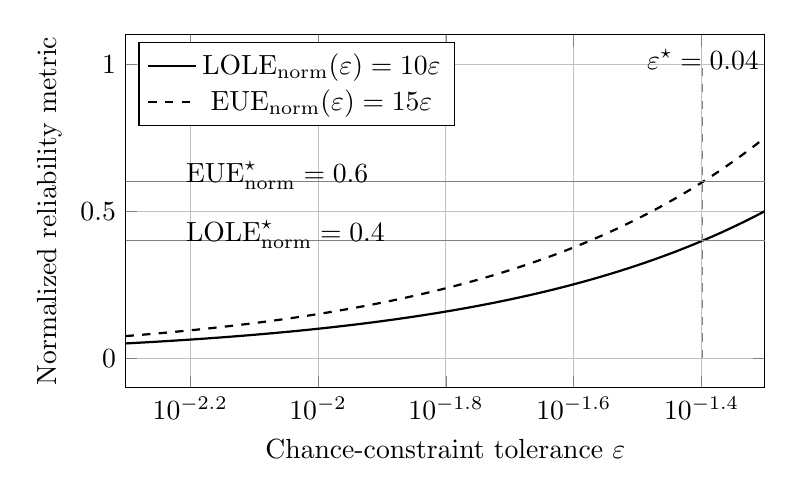
\begin{tikzpicture}
    \begin{axis}[
      width=0.8\textwidth,
      height=0.5\textwidth,
      xlabel={Chance-constraint tolerance $\varepsilon$},
      ylabel={Normalized reliability metric},
      xmin=0.005, xmax=0.05,
      xmode=log,
      grid=both,
      legend style={at={(0.02,0.98)},anchor=north west}
    ]
      % LOLE_norm(epsilon) = 10 * epsilon
      \addplot[thick, domain=0.005:0.05, samples=200]
        {10*x};
      \addlegendentry{$\LOLE_{\mathrm{norm}}(\varepsilon) = 10\varepsilon$};

      % EUE_norm(epsilon) = 15 * epsilon
      \addplot[thick, dashed, domain=0.005:0.05, samples=200]
        {15*x};
      \addlegendentry{$\EUE_{\mathrm{norm}}(\varepsilon) = 15\varepsilon$};

      % Target LOLE horizontal
      \addplot[thin, gray, domain=0.005:0.05] {0.4};
      \node[anchor=west] at (axis cs:0.006,0.42) {$\LOLE^\star_{\mathrm{norm}}=0.4$};

      % Target EUE horizontal
      \addplot[thin, gray, domain=0.005:0.05] {0.6};
      \node[anchor=west] at (axis cs:0.006,0.62) {$\EUE^\star_{\mathrm{norm}}=0.6$};

      % Epsilon* vertical
      \addplot[thin, gray, dashed] coordinates {(0.04,0) (0.04,1)};
      \node[anchor=south] at (axis cs:0.04,0.95) {$\varepsilon^\star=0.04$};
    \end{axis}
  \end{tikzpicture}
  \caption{Stylized calibration of the CED chance-constraint tolerance $\varepsilon$
  to normalized reliability metrics for a fixed portfolio $R$, with
  $\LOLE_{\mathrm{norm}}(\varepsilon)=10\varepsilon$ and
  $\EUE_{\mathrm{norm}}(\varepsilon)=15\varepsilon$. The reliability targets
  $(\LOLE^\star_{\mathrm{norm}},\EUE^\star_{\mathrm{norm}})=(0.4,0.6)$ are achieved
  at $\varepsilon^\star=0.04$.}
  \label{fig:eps_calibration}
\end{figure}

\section{Implications for ARQ and Resource Selection}

We briefly sketch implications for accelerated resource adequacy queue (ARQ) scoring.

\subsection{ARQ metrics}

In ARQ-style frameworks, candidate resources are ranked using metrics such as:
\begin{itemize}[leftmargin=*]
  \item net \$ per RA-MW (net cost per accredited MW of firm capacity),
  \item RA-MW per \$B (accredited MW per billion dollars),
  \item marginal \(-\Delta\EUE\) per \$/MW,
  \item survival probabilities for COD (commercial operation date) and deliverability factors.
\end{itemize}

Storage's ARQ score depends heavily on:
\begin{itemize}[leftmargin=*]
  \item its ability to mitigate scarcity in critical hours (as reflected in \(-\Delta\EUE\)),
  \item and the scarcity rents it can earn, which are linked to LMPs and bid caps.
\end{itemize}

\subsection{Bid caps and ARQ bias}

If storage bid caps are set:
\begin{itemize}[leftmargin=*]
  \item too low relative to risk-aware opportunity costs, storage scarcity rents are artificially suppressed; ARQ may undervalue storage relative to its MRV, biasing selection against it.
  \item too high, storage may appear overly profitable in simulations, leading ARQ to over-rank storage projects even if their actual contribution to \(-\Delta\EUE\) is modest.
\end{itemize}

By anchoring bid caps to risk-aware LMPs derived from CED and calibrating \(\varepsilon\) to reliability targets, ARQ analysis can:
\begin{itemize}[leftmargin=*]
  \item operate on a consistent scarcity pricing regime,
  \item ensure that simulated revenues and costs reflect \(\VOLL\)-aligned risk preferences,
  \item and avoid systematic bias in storage selection.
\end{itemize}

\begin{figure}[t]
  \centering
  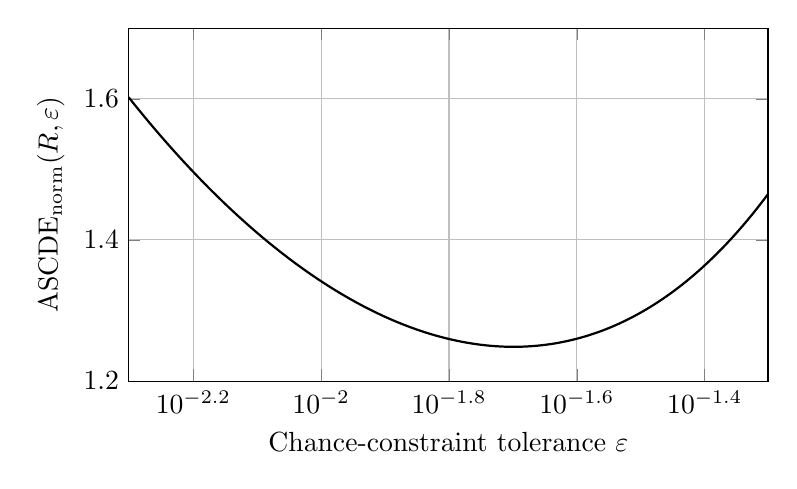
\begin{tikzpicture}
    \begin{axis}[
      width=0.8\textwidth,
      height=0.5\textwidth,
      xlabel={Chance-constraint tolerance $\varepsilon$},
      ylabel={$\ASCDE_{\mathrm{norm}}(R,\varepsilon)$},
      xmin=0.005, xmax=0.05,
      xmode=log,
      ymin=1.2, ymax=1.7,
      grid=both
    ]
      % ASCDE_norm(epsilon) = 0.4 + 0.08/sqrt(eps) + 14.1421*eps
      \addplot[thick, domain=0.005:0.05, samples=200]
        {0.4 + 0.08/sqrt(x) + 14.1421356237*x};
    \end{axis}
  \end{tikzpicture}
  \caption{Conceptual dependence of normalized ASCDE on the chance-constraint
  tolerance $\varepsilon$ for a fixed portfolio $R$, with
  $\ASCDE_{\mathrm{norm}}(\varepsilon) = 0.4 + 0.08/\sqrt{\varepsilon}
  + 14.1421\,\varepsilon$. The $0.08/\sqrt{\varepsilon}$ term captures higher
  operating cost under more conservative risk, while the linear term in
  $\varepsilon$ reflects the monetized reliability penalty proportional to
  $\EUE_{\mathrm{norm}}(\varepsilon)$.}
  \label{fig:ascde_vs_epsilon}
\end{figure}

\begin{figure}[t]
  \centering
  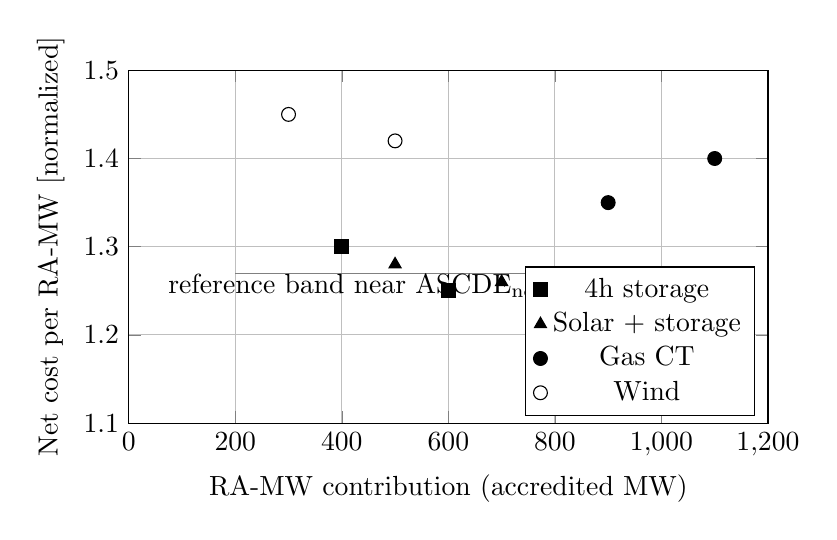
\begin{tikzpicture}
    \begin{axis}[
      width=0.8\textwidth,
      height=0.5\textwidth,
      xlabel={RA-MW contribution (accredited MW)},
      ylabel={Net cost per RA-MW [normalized]},
      xmin=0, xmax=1200,
      ymin=1.1, ymax=1.5,
      grid=both,
      legend style={at={(0.98,0.02)},anchor=south east}
    ]
      % 4h storage candidates (clustered near ASCDE_min)
      \addplot[only marks, mark=square*, mark size=2.5pt]
        coordinates {(400,1.30) (600,1.25) (800,1.23)};
      \addlegendentry{4h storage};

      % Solar + storage
      \addplot[only marks, mark=triangle*, mark size=2.5pt]
        coordinates {(500,1.28) (700,1.26)};
      \addlegendentry{Solar + storage};

      % Gas CT (higher net cost per RA-MW)
      \addplot[only marks, mark=*, mark size=2.5pt]
        coordinates {(900,1.35) (1100,1.40)};
      \addlegendentry{Gas CT};

      % Wind (lower RA-MW, higher cost per RA-MW)
      \addplot[only marks, mark=o, mark size=2.5pt]
        coordinates {(300,1.45) (500,1.42)};
      \addlegendentry{Wind};

      % Reference contour near ASCDE_min
      \addplot[thin, gray, domain=200:1100] {1.27};
      \node[anchor=north east] at (axis cs:1100,1.28)
        {reference band near $\ASCDE_{\mathrm{norm}}$ at $\varepsilon\approx 0.02$};
    \end{axis}
  \end{tikzpicture}
  \caption{Conceptual ARQ decision map showing candidate resources in a plane of
  reliability contribution (RA-MW) versus normalized net cost per RA-MW. The vertical
  scale is anchored near the minimum of $\ASCDE_{\mathrm{norm}}(R,\varepsilon)$ around
  $\varepsilon\approx 0.02$. Storage and solar+storage appear near the reference
  band, while gas CT and wind sit at higher net cost per RA-MW in this toy example.}
  \label{fig:arq_decision_map}
\end{figure}

\newpage

\section{Policy and Implementation Considerations}

We now translate the preceding analysis into a concrete policy and implementation roadmap for ISO/RTOs.

\subsection{Replacing heuristic storage caps}

Many ISO/RTOs currently use heuristic caps for storage offers, such as:
\begin{itemize}[leftmargin=*]
  \item a fixed multiple of average LMP,
  \item the 4th-highest LMP in a recent lookback window,
  \item or a generic system-wide cap equal to the overall price cap.
\end{itemize}
These heuristics are insensitive to:
\begin{itemize}[leftmargin=*]
  \item location,
  \item SoC,
  \item net-load uncertainty regime,
  \item and risk preference.
\end{itemize}

A transition pathway to Qi--Xu style caps:
\begin{enumerate}[leftmargin=*]
  \item \textbf{Uncertainty modeling.}
    Estimate net-load uncertainty and correlations across nodes and hours using historical data and forward-looking scenarios.
  \item \textbf{Choose a family of chance-constraint approximations.}
    For example, sub-Gaussian or unimodal distributionally robust bounds; document assumptions.
  \item \textbf{Risk posture calibration.}
    For the current portfolio, calibrate \(\varepsilon\) to approximate planning \(\LOLE^\star\) and \(\EUE^\star\) as outlined earlier.
  \item \textbf{CED and LMP envelopes.}
    Solve CED (or an approximate reduced form) to obtain risk-aware LMP distributions at each node and hour.
  \item \textbf{Construct SoC-dependent bid curves.}
    For each storage class and location, construct bid caps as functions of normalized SoC using the envelopes of risk-aware LMPs.
  \item \textbf{Codify and expose the mapping.}
    Publish the functional forms and parameters, with clear documentation of the uncertainty model and \(\varepsilon\).
\end{enumerate}

\subsection{Interaction with scarcity pricing}

If an ISO/RTO already employs scarcity pricing via operating reserve demand curves, there is an opportunity to align:
\begin{itemize}[leftmargin=*]
  \item the tails of \(\hat{\lambda}_{n,t}\),
  \item the peak of scarcity prices,
  \item and \(\VOLL\) used in \(\RA\).
\end{itemize}
Bid caps constructed from risk-aware LMPs should respect the scarcity pricing envelope; otherwise, storage may be structurally prevented from capturing scarcity rents that are, in principle, rational and desired for investment signaling.

\subsection{Telemetry and enforcement}

Implementing SoC-dependent caps requires:
\begin{itemize}[leftmargin=*]
  \item reliable real-time telemetry of storage SoC,
  \item robust validation of declared SoC at offer submission,
  \item and clear rules for how caps are applied when telemetry is lost or corrupted.
\end{itemize}
One practical approach is to:
\begin{itemize}[leftmargin=*]
  \item discretize normalized SoC into bands (e.g., 0--20\%, 20--40\%, etc.),
  \item pre-compute caps for each band and node,
  \item and enforce them via market software when offers are submitted.
\end{itemize}
If a unit's SoC changes between offer submission and dispatch, rules may specify conservative band choices to avoid over-allowing bids.

\section{Conclusion and Appendix Roadmap}

We have argued that locational, SoC-dependent storage bid bounds derived from chance-constrained dispatch provide a conceptually coherent and practically attractive way to manage storage offers in high-renewables, high-storage systems.
When embedded in an \(\ASCDE\)/UEVF perspective:
\begin{itemize}[leftmargin=*]
  \item bid caps are no longer arbitrary; they are tied to a risk posture that is itself calibrated to reliability targets,
  \item scarcity pricing, \(\VOLL\), \(\LOLE/\EUE\), and storage bid caps become different aspects of one stochastic optimization problem,
  \item and resource selection via ARQ can be conducted on a consistent basis with operational risk preferences.
\end{itemize}

To deepen the rigor and support regulatory and technical scrutiny, the following appendices are natural next steps.

\subsection*{Appendix roadmap}

\noindent
\textbf{Appendix A: Full CED primal--dual formulation.}
\begin{itemize}[leftmargin=*]
  \item Explicit primal formulation of CED with all constraints (energy, reserves, ramping, transmission).
  \item Dual derivation showing how risk-sensitive constraints map into LMPs and SoC shadow values.
  \item KKT conditions and complementary slackness structure for storage.
\end{itemize}

\noindent
\textbf{Appendix B: Distributionally robust chance constraints.}
\begin{itemize}[leftmargin=*]
  \item Formal definition of uncertainty sets (e.g., moment-based, unimodal).
  \item Derivation of \(\kappa(\varepsilon)\) for different robust regimes (Chebyshev, Gauss, etc.).
  \item Comparison of conservatism and computational tractability.
\end{itemize}

\noindent
\textbf{Appendix C: Stylized calibration of \(\varepsilon\) to \(\LOLE\).}
\begin{itemize}[leftmargin=*]
  \item Simple two-period or multi-period toy model linking \(\varepsilon\) to approximate \(\LOLE\) and \(\EUE\).
  \item Analytical expressions in special cases (e.g., single-node system with i.i.d.~load errors).
  \item Sensitivity of \(\LOLE\) to \(\varepsilon\) and uncertainty scale.
\end{itemize}

\noindent
\textbf{Appendix D: Example ISO implementation sketch.}
\begin{itemize}[leftmargin=*]
  \item Mapping the abstract framework to a specific market (e.g., MISO or CAISO) with current tariff structures.
  \item Pseudocode or high-level algorithm for computing bid caps on a daily or seasonal basis.
  \item Discussion of integration with existing market monitoring and mitigation rules.
\end{itemize}

\noindent
\textbf{Appendix E: Notation and symbol glossary.}
\begin{itemize}[leftmargin=*]
  \item Comprehensive table of all symbols used (\(\lambda,\theta,\varepsilon,\VOLL,\LOLE,\EUE,\ASCDE\), etc.).
  \item Cross-reference to sections and equations for quick navigation.
\end{itemize}

In subsequent drafts, these appendices can be populated with detailed derivations and case-study-style examples, turning the present conceptual treatment into a fully self-contained technical reference.

\section*{Acknowledgments}

This draft synthesizes and reinterprets results from Qi and Xu~\cite{QiXu2025} through the lens of reliability-aware resource valuation (\(\ASCDE\)/UEVF).
Any errors or misinterpretations remain the responsibility of the present author.

\newpage

\bibliographystyle{plainnat}
\begin{thebibliography}{9}

\bibitem{QiXu2025}
N.~Qi and B.~Xu.
\newblock Locational energy storage bid bounds for facilitating social welfare convergence.
\newblock \emph{IEEE Transactions on Energy Markets, Policy and Regulation}, 2025.
\newblock Also available as arXiv:2502.18598.

\bibitem{RockafellarUryasev2000}
R.~T. Rockafellar and S.~Uryasev.
\newblock Optimization of conditional value-at-risk.
\newblock \emph{Journal of Risk}, 2(3):21--41, 2000.

\bibitem{ShapiroDentchevaRuszczynski}
A.~Shapiro, D.~Dentcheva, and A.~Ruszczynski.
\newblock \emph{Lectures on Stochastic Programming: Modeling and Theory}.
\newblock SIAM, 2009.

\end{thebibliography}

\newpage

% --- Appendices ---

\appendix

\section{Chance-Constrained Economic Dispatch: Full Primal--Dual Formulation}
\label{app:ced-full}

This appendix provides a more explicit primal--dual formulation of the chance-constrained economic dispatch (CED) problem underlying the risk-aware LMPs and storage bid bounds.

\subsection{Network and resource model}

We consider a DC network with:
\begin{itemize}[leftmargin=*]
  \item nodes \(n \in \mathcal{N}\),
  \item transmission lines \(\ell \in \mathcal{L}\),
  \item generators \(i \in G\) with node mapping \(n(i)\),
  \item storage units \(s \in S\) with node mapping \(n(s)\).
\end{itemize}
For simplicity, we restrict attention to energy-only dispatch with reserves implicit in ramping and capacity limits, but the structure extends to explicit reserve variables.

Let:
\begin{itemize}[leftmargin=*]
  \item \(g_{i,t}\) be generator output,
  \item \(p_{s,t}\), \(b_{s,t}\) be storage discharge and charge,
  \item \(e_{s,t}\) be storage SoC,
  \item \(f_{\ell,t}\) be line flow,
  \item \(\theta_{n,t}^{\text{ang}}\) be voltage angle at node \(n\),
  \item \(\tilde{d}_{n,t}\) be stochastic net load.
\end{itemize}
The PTDF matrix is denoted \(H \in \RR^{|\mathcal{L}| \times |\mathcal{N}|}\), with rows \(H_\ell\).

\subsection{Primal CED formulation}

For a given realization of net load (mean plus uncertainty), the CED problem is:
\begin{equation}
  \begin{aligned}
  \min_{g,p,b,e,f,\theta^{\text{ang}}}
  \quad
  & \sum_{t=1}^T \left( \sum_{i \in G} C_i(g_{i,t}) + \sum_{s \in S} M_s (p_{s,t} + b_{s,t}) \right) \\
  \text{s.t.}\quad
  & \textbf{(Node balance)}\quad
  \sum_{i \in G_n} g_{i,t}
  + \sum_{s \in S_n} (p_{s,t} - b_{s,t})
  - \tilde{d}_{n,t}
  = \sum_{\ell \in \mathcal{L}_n} f_{\ell,t},
  \ \forall n,t, \\
  & \textbf{(DC flows)}\quad
  f_{\ell,t} = H_\ell^\top \theta^{\text{ang}}_{\cdot,t},
  \ \forall \ell,t, \\
  & \textbf{(Line limits)}\quad
  -\overline{F}_\ell \le f_{\ell,t} \le \overline{F}_\ell, \ \forall \ell,t, \\
  & \textbf{(Gen limits)}\quad
  \underline{g}_i \le g_{i,t} \le \overline{g}_i,\ \forall i,t, \\
  & \textbf{(Ramps)}\quad
  -R_i \le g_{i,t} - g_{i,t-1} \le R_i,\ \forall i,t>1, \\
  & \textbf{(SoC dynamics)}\quad
  e_{s,t+1} = e_{s,t} + \eta_s b_{s,t} - \frac{1}{\eta_s} p_{s,t},\ \forall s,t, \\
  & \underline{e}_s \le e_{s,t} \le \overline{e}_s,\ \forall s,t, \\
  & 0 \le b_{s,t} \le \overline{b}_s, \quad 0 \le p_{s,t} \le \overline{p}_s,\ \forall s,t, \\
  & \textbf{(Reference angle)}\quad
  \theta^{\text{ang}}_{n_{\mathrm{ref}},t} = 0,\ \forall t, \\
  & \textbf{(Chance constraints)}\quad
  \PP\big( \mathcal{C}_k(g,p,b,e,f,\tilde{d}) \le 0 \big) \ge 1-\varepsilon,\ \forall k \in \mathcal{K}.
  \end{aligned}
  \label{eq:CED-raw}
\end{equation}
Here \(\mathcal{C}_k\) denote generic constraints sensitive to uncertainty (e.g., line limits, reserves).

\subsection{Deterministic reformulation via DRCC}

Each chance constraint \(k\) has the form:
\[
  \PP(a_k^\top x + c_k^\top \tilde{z} \le b_k) \ge 1-\varepsilon,
\]
where:
\begin{itemize}[leftmargin=*]
  \item \(x = (g,p,b,e,f,\theta^{\text{ang}})\),
  \item \(\tilde{z}\) collects uncertainty terms (deviations of net load from mean).
\end{itemize}
Under a chosen distributionally robust or parametric model (Appendix~\ref{app:drcc}), we obtain a deterministic approximation:
\[
  a_k^\top x + \kappa_k(\varepsilon) \sigma_k(x) \le b_k,
\]
where \(\sigma_k(x)\) is an effective standard deviation or uncertainty norm.

Substituting these approximations yields a deterministic convex program:
\begin{equation}
  \begin{aligned}
  \min_{x} \quad & c^\top x \\
  \text{s.t.}\quad & A x \le b, \\
                   & A^{\mathrm{DR}}(\varepsilon) x \le b^{\mathrm{DR}}(\varepsilon),
  \end{aligned}
  \label{eq:CED-det}
\end{equation}
where \(A\) collects deterministic network and operational constraints, and \(A^{\mathrm{DR}}(\varepsilon)\) encodes DRCC-based tightened constraints.

\subsection{Dual problem and LMPs}

Let \(\lambda\) collect dual variables for nodal balance, \(\pi\) for line limits, \(\alpha,\beta\) for generator bounds, \(\rho\) for ramps, \(\mu^\pm\) for SoC bounds, and \(\phi\) for DRCC constraints.
The dual problem associated with~\eqref{eq:CED-det} can be written as:
\begin{equation}
  \begin{aligned}
  \max_{\lambda,\pi,\alpha,\beta,\rho,\mu^\pm,\phi}
  \quad
  & -b^\top y - (b^{\mathrm{DR}}(\varepsilon))^\top \phi \\
  \text{s.t.}\quad
  & A^\top y + (A^{\mathrm{DR}}(\varepsilon))^\top \phi + c = 0, \\
  & y \ge 0,\ \phi \ge 0,
  \end{aligned}
  \label{eq:CED-dual}
\end{equation}
where \(y\) collects primary duals (including nodal balances).

The LMP at node \(n\), time \(t\), is the dual \(\hat{\lambda}_{n,t}\) associated with nodal balance at that node/time.
Shadow prices associated with SoC dynamics are contained in a subset of dual variables; we denote them \(\hat{\theta}_{s,t}\), interpreted as marginal values of energy in storage at time \(t\).

Complementarity conditions link:
\begin{itemize}[leftmargin=*]
  \item binding line constraints to congestion components of LMPs,
  \item binding DRCC constraints to scarcity premia induced by uncertainty and risk,
  \item SoC dynamics to storage's intertemporal opportunity costs.
\end{itemize}

\section{Distributionally Robust Chance Constraints}
\label{app:drcc}

We briefly outline several DRCC formulations relevant to CED and derive corresponding \(\kappa(\varepsilon)\) factors.

\subsection{Moment-based Chebyshev/Cantelli bounds}

Consider a scalar random variable \(Y\) with mean \(\mu_Y\) and variance \(\sigma_Y^2\).
Chebyshev's inequality gives:
\[
  \PP(|Y - \mu_Y| \ge t) \le \frac{\sigma_Y^2}{t^2}.
\]
Cantelli's inequality tightens the one-sided case:
\[
  \PP(Y - \mu_Y \ge t) \le \frac{\sigma_Y^2}{\sigma_Y^2 + t^2}.
\]
Solving for \(t\) in \(\PP(Y \le \mu_Y + t) \ge 1-\varepsilon\) yields:
\begin{equation}
  t \ge \sigma_Y \sqrt{ \frac{1-\varepsilon}{\varepsilon} }.
\end{equation}
Thus, for a linear functional of uncertainty \(Y = c^\top \tilde{z}\), we can approximate:
\begin{equation}
  \PP(a^\top x + Y \le b) \ge 1-\varepsilon
  \ \Longleftarrow\
  a^\top x + \sigma_Y \sqrt{\tfrac{1-\varepsilon}{\varepsilon}} \le b.
\end{equation}
This motivates a DRCC coefficient:
\begin{equation}
  \kappa(\varepsilon) = \sqrt{\frac{1-\varepsilon}{\varepsilon}}.
\end{equation}

\subsection{Gaussian case}

If we assume \(\tilde{z} \sim \mathcal{N}(0,\Sigma)\), then \(Y = c^\top \tilde{z} \sim \mathcal{N}(0, \sigma_Y^2)\) with \(\sigma_Y = \sqrt{c^\top \Sigma c}\).
The chance constraint
\[
  \PP(a^\top x + Y \le b) \ge 1-\varepsilon
\]
is equivalent to:
\begin{equation}
  a^\top x + \Phi^{-1}(1-\varepsilon) \sigma_Y \le b,
\end{equation}
where \(\Phi\) is the standard normal CDF.
Thus \(\kappa(\varepsilon) = \Phi^{-1}(1-\varepsilon)\).

\subsection{Unimodal distributions}

When only unimodality and second moments are known, tighter than Chebyshev but looser than Gaussian bounds can be obtained (e.g., via Gauss or Vysochanski\u{\i}--Petunin inequalities).
Qi and Xu consider several such settings and tabulate corresponding \(\kappa(\varepsilon)\) values.
The general template remains:
\begin{equation}
  a^\top x + \kappa(\varepsilon) \sqrt{c^\top \Sigma c} \le b.
\end{equation}
More conservative choices of \(\kappa(\varepsilon)\) yield lower violation probabilities at the cost of increased dispatch conservatism and higher risk-aware LMPs.

\subsection{Vector-valued DRCC}

For multiple correlated constraints, DRCC can be defined over an uncertainty set:
\[
  \mathcal{U} = \{ z \in \RR^m : z^\top \Sigma^{-1} z \le \gamma \},
\]
with some radius \(\gamma\).
Then the worst-case realization of \(c^\top z\) subject to \(z \in \mathcal{U}\) is:
\begin{equation}
  \max_{z: z^\top \Sigma^{-1} z \le \gamma} c^\top z
  = \sqrt{\gamma}\, \sqrt{c^\top \Sigma c}.
\end{equation}
Hence a DRCC of the form:
\[
  a^\top x + \sqrt{\gamma} \sqrt{c^\top \Sigma c} \le b,
\]
with \(\gamma\) chosen to correspond to a desired violation probability under an assumed elliptical distribution.
This generalizes the scalar cases above.

\section{Calibration of \texorpdfstring{\(\varepsilon\)}{epsilon} to Reliability Metrics}
\label{app:calibration}

To make the link between the CED risk parameter \(\varepsilon\) and reliability metrics concrete, we present a stylized one-node, two-period example.

\subsection{Two-period single-node model}

Consider:
\begin{itemize}[leftmargin=*]
  \item one node, one generator with capacity \(G\), no storage,
  \item two periods \(t=1,2\),
  \item net loads \(\tilde{L}_1, \tilde{L}_2\) with means \(L_1,L_2\) and zero-mean deviations \(\tilde{z}_1,\tilde{z}_2\).
\end{itemize}
Assume:
\begin{itemize}[leftmargin=*]
  \item generator can be pre-committed to capacity \(G\) in both periods,
  \item any unmet load becomes unserved energy at cost \(\VOLL\),
  \item chance constraints impose \(\PP(\tilde{L}_t \le G) \ge 1-\varepsilon\), \(t=1,2\).
\end{itemize}

\subsection{Chance constraints and LOLE}

Assume for simplicity that \(\tilde{L}_t = L_t + \tilde{z}_t\) with \(\tilde{z}_t \sim \mathcal{N}(0,\sigma^2)\) i.i.d.
Then:
\begin{equation}
  \PP(\tilde{L}_t \le G)
  = \PP\left( \frac{\tilde{L}_t - L_t}{\sigma} \le \frac{G - L_t}{\sigma} \right)
  = \Phi\left(\frac{G - L_t}{\sigma}\right).
\end{equation}
Imposing:
\[
  \Phi\left(\frac{G - L_t}{\sigma}\right) \ge 1-\varepsilon
\]
is equivalent to:
\begin{equation}
  \frac{G - L_t}{\sigma} \ge \Phi^{-1}(1-\varepsilon)
  \quad\Rightarrow\quad
  G \ge L_t + \sigma \Phi^{-1}(1-\varepsilon).
\end{equation}
To satisfy this for both \(t=1,2\), we need:
\begin{equation}
  G \ge \max_t \Big( L_t + \sigma \Phi^{-1}(1-\varepsilon) \Big).
\end{equation}

The LOLE (in hours) is:
\begin{equation}
  \LOLE = \sum_{t=1}^2 \PP(\tilde{L}_t > G)
  = \sum_{t=1}^2 \big( 1 - \Phi\big( (G-L_t)/\sigma \big) \big).
\end{equation}
If \(G\) is chosen just at the chance-constraint threshold, then:
\begin{equation}
  \PP(\tilde{L}_t > G) \le \varepsilon,\quad t=1,2,
\end{equation}
and hence:
\begin{equation}
  \LOLE \le 2\varepsilon.
\end{equation}
Thus, in this toy model, \(\varepsilon\) controls LOLE approximately linearly:
\[
  \varepsilon \approx \frac{\LOLE}{2}.
\]

\subsection{EUE in the toy model}

Assuming the same normal structure, expected unserved energy in period \(t\) is:
\begin{equation}
  \EE[(\tilde{L}_t - G)_+]
  = \int_{G}^{\infty} (x-G) \frac{1}{\sigma\sqrt{2\pi}} 
      \exp\left( -\frac{(x-L_t)^2}{2\sigma^2} \right)\, dx.
\end{equation}
Closed-form expressions exist in terms of \(\Phi\) and \(\phi\) (density) for truncated normal expectations.
One obtains:
\begin{equation}
  \EE[(\tilde{L}_t - G)_+]
  = \sigma \phi\left(\frac{G-L_t}{\sigma}\right) 
    - (G-L_t) \big(1-\Phi((G-L_t)/\sigma)\big).
\end{equation}
At the chance-constraint threshold, \(G-L_t = \sigma \Phi^{-1}(1-\varepsilon)\), we can evaluate this explicitly as a function of \(\varepsilon\).
Summing over \(t\) gives \(\EUE(\varepsilon)\).

Though simplistic, this illustrates:
\begin{itemize}[leftmargin=*]
  \item chance constraint tolerance \(\varepsilon\) controls LOLE and EUE in an explicit way,
  \item smaller \(\varepsilon\) implies larger \(G\), lower LOLE/EUE, and higher capacity cost.
\end{itemize}
In richer multi-node, multi-period models, the relationship is more complex but conceptually similar: \(\varepsilon\) tunes the tail probability of violating adequacy constraints, which maps into LOLE and EUE via the system's joint distribution of net load and contingencies.

\section{Implementation Sketch for an ISO/RTO}
\label{app:implementation}

We outline a practical high-level implementation pipeline for an ISO/RTO integrating Qi--Xu-style bid bounds into an \(\ASCDE\)/UEVF-consistent framework.

\subsection{Offline analysis and parameter calibration}

\begin{enumerate}[leftmargin=*]
  \item \textbf{Data assembly.}
    Gather:
    \begin{itemize}
      \item historical net-load time series at nodal or zonal resolution,
      \item renewable output and forecast error distributions,
      \item generator outage statistics,
      \item storage fleet characteristics (power, energy, efficiencies).
    \end{itemize}

  \item \textbf{Uncertainty modeling.}
    Estimate:
    \begin{itemize}
      \item mean net-load profiles \(d_{n,t}\),
      \item covariance matrix \(\Sigma\) (or suitable low-rank factorization) for net-load forecast errors across nodes and times,
      \item any relevant higher-moment or shape constraints (e.g., unimodality) needed for DRCC.
    \end{itemize}

  \item \textbf{Choice of DRCC regime.}
    Select:
    \begin{itemize}
      \item a family of DRCC approximations (Gaussian, Chebyshev, unimodal),
      \item corresponding \(\kappa(\varepsilon)\) functions.
    \end{itemize}
    Document assumptions and conservatism.

  \item \textbf{Risk posture calibration.}
    Using current or planned portfolio \(R\):
    \begin{itemize}
      \item for a grid of \(\varepsilon\) values, run Monte Carlo simulations of net-load and contingencies,
      \item for each draw, dispatch using CED with that \(\varepsilon\),
      \item compute empirical LOLE(\(R,\varepsilon\)) and EUE(\(R,\varepsilon\)),
      \item choose \(\varepsilon^\star\) such that LOLE and EUE are near planning targets.
    \end{itemize}

  \item \textbf{Risk-aware LMP envelopes.}
    For \(\varepsilon^\star\), construct:
    \begin{itemize}
      \item risk-aware LMP distributions \(\hat{\lambda}_{n,t}\) across Monte Carlo draws,
      \item SoC shadow values \(\hat{\theta}_{s,t}\) for storage units,
      \item summary statistics (e.g., upper and lower quantiles) at each node/time.
    \end{itemize}

  \item \textbf{SoC-dependent bid curves.}
    For each storage class (e.g., duration, technology) and location:
    \begin{itemize}
      \item discretize normalized SoC \(\xi \in [0,1]\) into bands,
      \item for each band, compute approximate max/min of \(\hat{A}_{s,t},\hat{B}_{s,t}\) across scenarios,
      \item fit smooth, monotone bid-cap curves \(\bar{A}_{s,t}(\xi)\), \(\bar{B}_{s,t}(\xi)\) that respect chance constraints.
    \end{itemize}
\end{enumerate}

\subsection{Operational integration}

\begin{enumerate}[leftmargin=*]
  \item \textbf{Cap tables.}
    For each day/season and node \(n\):
    \begin{itemize}
      \item publish tables of bid caps as a function of SoC band and time block (e.g., hourly, block-wise),
      \item update when material changes in uncertainty or risk posture occur.
    \end{itemize}

  \item \textbf{Offer validation.}
    For each storage offer:
    \begin{itemize}
      \item retrieve declared or telemetered SoC and location,
      \item map to the appropriate SoC band and node,
      \item enforce \(\text{offer price} \le \bar{A}_{s,t}(\text{band})\) for discharge segments and analogous for charge segments,
      \item flag and reject any bids exceeding caps, or route them to mitigation review.
    \end{itemize}

  \item \textbf{Market clearing.}
    Run standard day-ahead and real-time market clearing with:
    \begin{itemize}
      \item storage offers truncated by caps,
      \item risk-aware dispatch or conservative operating reserves consistent with \(\varepsilon^\star\).
    \end{itemize}

  \item \textbf{Ex-post analysis.}
    Periodically:
    \begin{itemize}
      \item compare realized LMPs, storage dispatch, and scarcity events with model predictions,
      \item update uncertainty models and, if necessary, recalibrate \(\varepsilon^\star\),
      \item reassess consistency between scarcity prices, \(\VOLL\), and reliability metrics.
    \end{itemize}
\end{enumerate}

\subsection{Regulatory and stakeholder communication}

The ISO/RTO should:
\begin{itemize}[leftmargin=*]
  \item publish technical documentation of the DRCC regime, \(\varepsilon\) calibration, and cap construction,
  \item explain how bid caps support reliability targets and avoid arbitrary price suppression,
  \item provide tools (e.g., public data sets and code snippets) for external analysts to replicate simplified variants.
\end{itemize}

\section{Notation and Symbol Glossary}
\label{app:notation}

Tables~\ref{tab:sets} and~\ref{tab:notation} summarize the main sets and symbols.

\begin{longtable}{@{}llp{8cm}@{}}
\caption{Index sets and entities}
\label{tab:sets}\\
\toprule
Symbol & Type & Description \\
\midrule
\endfirsthead
\toprule
Symbol & Type & Description \\
\midrule
\endhead
\bottomrule
\endfoot
\(\mathcal{T}\) & Set & Time periods (e.g., hours, \(t = 1,\dots,T\)) \\
\(\mathcal{N}\) & Set & Network nodes/buses \\
\(\mathcal{L}\) & Set & Transmission lines \\
\(G\) & Set & Conventional generators \\
\(S\) & Set & Storage units \\
\(\mathcal{K}\) & Set & Indexed chance-constrained constraints \\
\(\Omega\) & Set & Scenario space for uncertainty \(\omega\) \\
\(\mathcal{R}_{\mathrm{feasible}}\) & Set & Feasible resource portfolios \(R\) \\
\bottomrule
\end{longtable}

\begin{longtable}{@{}llp{8cm}@{}}
\caption{Variables and parameters}
\label{tab:notation}\\
\toprule
Symbol & Type & Description \\
\midrule
\endfirsthead
\toprule
Symbol & Type & Description \\
\midrule
\endhead
\bottomrule
\endfoot
\(g_{i,t}\) & Var. & Output of generator \(i \in G\) at time \(t\) (MW) \\
\(p_{s,t}\) & Var. & Discharge power of storage unit \(s \in S\) at time \(t\) (MW) \\
\(b_{s,t}\) & Var. & Charge power of storage unit \(s\) at time \(t\) (MW) \\
\(e_{s,t}\) & Var. & State of charge of storage unit \(s\) at time \(t\) (MWh) \\
\(\xi_{s,t}\) & Var. & Normalized SoC, \(\xi_{s,t} \in [0,1]\) \\
\(f_{\ell,t}\) & Var. & Flow on line \(\ell\) at time \(t\) (MW) \\
\(\theta^{\text{ang}}_{n,t}\) & Var. & Voltage angle at node \(n\), time \(t\) (rad) \\
\(\tilde{d}_{n,t}\) & RV & Random net load at node \(n\), time \(t\) (MW) \\
\(d_{n,t}\) & Param. & Mean net load at node \(n\), time \(t\) (MW) \\
\(\tilde{z}_{n,t}\) & RV & Net-load deviation, \(\tilde{d}_{n,t}-d_{n,t}\) (MW) \\
\(\Sigma\) & Param. & Covariance matrix of net-load deviations \\
\(C_i(\cdot)\) & Param. & Cost function of generator \(i\) (\$/MWh) \\
\(M_s\) & Param. & Degradation cost for storage \(s\) (\$/MWh) \\
\(\eta_s\) & Param. & Storage efficiency (round-trip or split) \\
\(\underline{g}_i,\overline{g}_i\) & Param. & Min/max output of generator \(i\) (MW) \\
\(R_i\) & Param. & Ramp limit of generator \(i\) (MW per period) \\
\(\underline{e}_s,\overline{e}_s\) & Param. & Min/max SoC of storage \(s\) (MWh) \\
\(\overline{b}_s,\overline{p}_s\) & Param. & Max charge/discharge power (MW) \\
\(\overline{F}_\ell\) & Param. & Line \(\ell\) thermal limit (MW) \\
\(H\) & Param. & PTDF matrix for DC power flows \\
\(\lambda_{n,t}\) & Dual & LMP at node \(n\), time \(t\) (deterministic ED) \\
\(\hat{\lambda}_{n,t}\) & Dual & Risk-aware LMP at node \(n\), time \(t\) (CED) \\
\(\theta_{s,t}\) & Dual & SoC shadow value for storage \(s\) at time \(t\) (deterministic ED) \\
\(\hat{\theta}_{s,t}\) & Dual & Risk-aware SoC shadow value (CED) \\
\(A_{s,t}\) & Def. & Marginal discharge cost, \(M_s + \theta_{s,t}/\eta_s\) (\$/MWh) \\
\(B_{s,t}\) & Def. & Marginal charge cost, \(\theta_{s,t}\eta_s - M_s\) (\$/MWh) \\
\(\hat{A}_{s,t}\) & Def. & Risk-aware marginal discharge cost (\$/MWh) \\
\(\hat{B}_{s,t}\) & Def. & Risk-aware marginal charge cost (\$/MWh) \\
\(\bar{A}_{s,t}\) & Param. & Discharge bid cap for storage \(s\), time \(t\) (\$/MWh) \\
\(\bar{B}_{s,t}\) & Param. & Charge bid cap for storage \(s\), time \(t\) (\$/MWh) \\
\(\varepsilon\) & Param. & Chance-constraint violation tolerance (risk parameter) \\
\(\kappa(\varepsilon)\) & Param. & Risk-sensitivity coefficient in DRCC approximation \\
\(\VOLL\) & Param. & Value-of-lost-load (\$/MWh) \\
\(\LOLE\) & Metric & Loss-of-load expectation (e.g., hours/year or days/year) \\
\EUE & Metric & Expected unserved energy (MWh/year) \\
\(\RA(R)\) & Metric & Monetized reliability cost for portfolio \(R\) (\$/year) \\
\(\ELCC_r\) & Metric & Effective load-carrying capability of resource \(r\) \\
\(\ASCDE(R,\varepsilon)\) & Metric & System-aware cost of dependable energy for portfolio \(R\) under risk \(\varepsilon\) (\$/MWh) \\
\(\mathrm{MRV}_r\) & Metric & Marginal reliability value of resource \(r\) (\$/MW-year) \\
\bottomrule
\end{longtable}

\end{document}